%%class
\documentclass{iaesarticle3}

%%required package. add for your convenient, but do not remove the initial
\usepackage{amsmath, amsfonts, amssymb, float, fancyhdr}
\usepackage[scaled]{uarial}
\usepackage[figuresright]{rotating}
\usepackage{authblk, graphicx, indentfirst, lastpage, lipsum}
\setlength{\affilsep}{0cm}
\renewcommand\Authfont{\normalsize}
\renewcommand\Affilfont{\normalfont\small}
\usepackage{subfig, caption, epstopdf}
\usepackage[left=3cm, right=3cm, top=3cm, bottom=3cm, includefoot]{geometry}
\usepackage{caption}
\captionsetup{labelsep=period}
\usepackage{titlesec}
\usepackage{lmodern}
\titleformat{\section}
  {\normalfont\normalsize\bfseries}{\thesection}{1em}{}
\titlespacing*{\section}{0cm}{0.7cm}{0cm}
\titlespacing*{\subsection}{0cm}{0.5cm}{0cm}

%%leave copyright info to the editor
\CopyrightLine[Copyright]{2013}{Universitas Ahmad Dahlan. All rights reserved.}

%%author
\author[*]{\bfseries Ayu Anggara}
\author[ ]{\bfseries M. Yusril Helmi Setyawan}
%%author's affiliation
\affil[ ]{Applied Bachelor Program of Informatics Engineering, Politeknik Pos Indonesia}
\affil[ ]{Bandung Indonesia, Phone. 022-2009562, 2009570 Fax. 022-2009568}
\affil[*]{Ayu Anggara, e-mail: ayuanggaraspentwo@gmail.com}

%%title and shortitle (for footer)
\title{Implementation of Multi-Factor Authentication Method to Minimize RFID Duplication.}
\shorttitle{Open Presences System Design (Ayu Anggara)}

%%starting
\begin{document}

%%indentation. do not change
\setlength{\parindent}{1.27cm}

%%header and footer setting. do not change
\pagestyle{fancy}
\fancyhfoffset{0cm}

%%journal info
\journalname{TELKOMNIKA Indonesian Journal of Electrical Engineering}
\journalshortname{TELKOMNIKA}
\revhistory{Received May 9, 201x; Revised August 3, 201x; Accepted August 16, 201x}
\vol{x}
\no{x}
\doi{10.11591/telkomnika.vXiY.abcd}
\months{April}
\years{2013}
\issn{2302-4046}

%%build title
\maketitle


\begin{abstract}
\textit{\indent}
RFID technology is an automatic wireless identification system that works with the help of active and passive cards as well as with the reader. The use of unique numbers inside RFID tags is very useful as the identity of an object or as a tracking device. As for weaknesses in RFID systems, it is possible to cloning identification data. Therefore it is necessary to increase security to minimize it. Authentication is the process of user verification. The most common form of Authentication is single-factor Authentication, which requires only one factor for users to log in to the system. This model is weak and can cause harm to those who use it. Therefore Multi-factor Authentication is required that is the way to authenticate users by using multiple layers of Authentication program. The factor to be used in this report is to use One-Time Password. With the system with several steps of this authentication can also minimize the fraud that will occur. As the proxy case absent and minimize the occurrence of duplication of RFID card
\end{abstract}

\begin{keyword}
\textit{}
RFID, Multi-Factor Authentication, One-Time Password, Duplication
\end{keyword}

\section{Introduction}
\label{Introduction}
At present, Many industries today are using Radio Frequency Identification (RFID) technology \cite{Zaman2017}, RFID applies in applications such as attendance logging applications \cite{Eridani2015}, warehouse management \cite{xie2014efficiently}, library \cite{liu2017rf}, object tracking \cite{bu2015deterministic}, and others. RFID can create objects of "talking" technology, so RFID technology in key technologies from perceptual perception layer positions is very prominent \cite{pane2018qualitative}. RFID has several advantages over the traditional identification technologies. RFID does not require random tracks for communication and RFID tags can be read more \cite{Arjona2015}. RFID is relatively fast, and many tags can read simultaneously. The RFID system consists of RFID tags, RFID reader and PC \cite{Almaaitah2014}. Each of RFID tag has a unique ID that corresponds to some useful information (e.g. product, tracking, and position information), from unique ID and position information, users can quickly identify RFID tag locations \cite{Xu2016}.\par
While RFID widely use, it is important to note that RFID has weaknesses. The weakness in RFID systems is that it is possible to clone identification data \cite{basilio2016multifactor}. Cloning attacks make the application unsafe because it duplicates the original tags so that it threatens RFID applications that use tag authenticity to validate objects \cite{maleki2017new}. This cloning attack can result in financial loss to users \cite{shao2015protar}, \cite{huang2017dtd}.\par
Therefore, to improve system security and minimise duplication in RFID system in this research will apply Multi-Factor Authentication (MFA) method. MFA is a way to authenticate users by using multiple layers of the Authentication program. This is a secure means of authentication that can effectively prevent identity theft \cite{Venukumar2016}. In addition, using this method will be slavish in tracking the precision of the calculation of the tracking results \cite{Awangga2017}. The factor in this report is using One-Time Password (OTP). Thus, the existence of a system with some authentication steps can minimise the fraud and duplication that will occur \cite{jacob2015mobile}.


\section{RelatedWork}
\label{Related Work}
Applications that use Radio Frequency Identification (RFID) are increasing today and are seen applicable in areas such as material flow discharge, quality assurance \cite{marcus2017system}, production control \cite{ramadan2017rfid}, \cite{tao2017advanced}, cold chain logistics tracking \cite{chen2014novel}, objects in place of find \cite{cai2014boundary}. RFID consists of two important parts of the RFID reader (combination of transceiver and antenna) and RFID tags (composed of unique numbers). The RFID tag is used to store important data from the observer while the reader is used to read the data stored in the tag. This technology has the advantage of data transfer that is contactless and able to work in every environment \cite{wang2017deep}. RFID is one of the wireless technologies that use electromagnetic signal detection as identification \cite{abas2017attendance}. Frequencies used in RFID consist of various types of frequencies such as low frequency, high frequency, ultra high frequency, and microwave \cite{srinidhi2015web}. In particular, referring to the process tracer category of the process, researchers mainly focus on manufacturing, production logistics, inventory, and supply chain. At an in-place level, RFID improves real-time data retrieval and fuses for process visibility. Propose a formal RFID-based deduction model to monitor changes in the flow of time-sensitive materials in the workshop \cite{cao2017real}. Most existing cloning detection protocols are suitable for recognisable systems, requiring knowledge of tag IDs. Such protocols to recognise IDs before detecting which IDs are related to the cloning tag and focus only on the RFID supply chain; they collect IDs from supply chain partners and detect cloned attacks when the IDs appear simultaneously in different places \cite{kang2013development}.\par
Authentication is one of the critical aspects of securing applications and systems. During the authentication process, Biometric and RFID are validation factors for verifying user identity \cite{basilio2016multifactor}, Combining user location with username and password as Multi-Factor Authentication (MFA) system to make authentication more secure \cite{Ramatsakane2017}. For secure authentication of e-voting systems using cryptographic and fingerprint IC and FTP MFA techniques \cite{oke2017developing}, Schemes using cryptography and Android enhance security, convenience, flexibility, storage efficiency and MFA performance \cite{Venukumar2016}. Using a phrase-based MFA framework to make resources on the cloud safer \cite{rehman2016framework}. By implementing several MFAs on the mobile cloud, it is possible to know the feasibility of applying the method \cite{alizadeh2014feasibility}. Hardware authentication with Fingerprint and Smartphone \cite{ba2017addressing}, as well as a combination of passwords with hybrid profiles of user behaviour with a great combination of host-based features, are also to keep user data secure \cite{uluagac2014multi}. Utilization of MFA to minimise fraud attendance data such as using face-recognising \cite{sarker2016design}, Cloud verification system that combines biometric factors and Passwords to achieve high levels of security \cite{khan2015multi}. User database on API device information that can provide that information to web applications \cite{mandyam2015leveraging}. The MFA architecture utilises Identity Federation and Single-Sign-On technologies, for the modular integration of the authentication factor \cite{shah2015multi}. Authentication security is assured because of the nature of the hash function, the combination of secret vital methods and the method of creating a one-time token \cite{zhao2015asynchronous}. Merging NFC and One Time Password (OTP) methods to improve system security and eliminate attendance cheating \cite{jacob2015mobile}. NFC-based MFA systems have better security advantages with a simple login process \cite{hufstetler2017nfc}. 
\par Based on previous research, this research will do the design to improve the security of existing attendance system. The design will use Radio Frequency Identification (RFID) card as a tool of attendance by applying Multi-Factor Authentication method. MFA is a way to authenticate users by using multiple layers of authentication programs. One example is to use OTP (One-Time Password). OTP send to each user's mobile device; this OTP is only valid for one login session or transaction and, each user has a different OTP. Thus, using the MFA and OTP method can minimise the occurrence of fraud or duplication of attendance records system.


\section{Research Method}
\label{ResearchMethod}
In this study, the researchers combine the application of RFID and OTP (One-Time Password) authentication algorithm to achieve reliable Multi-Factor Authentication (MFA) method technique.

\subsection{Multi-Factor Authentication}
Multi-factor authentication (MFA) is a security approach for using more than one authentication tool from the available independent credentials to verify users. Multi-factor authentication combines two or more layers of the Authentication program: what users know (keywords), what users have (security tokens) and (biometric verification) \cite{oke2017developing}. The purpose of the MFA is to create layered defences and make it more difficult for unauthorised people to access targets such as physical locations, computing devices, networks or databases. If one factor is compromised or damaged, the attacker still has at least one more barrier to be broken before successfully breaking the target. This is widely known as the most secure method for authenticating access to data or applications \cite{shah2015multi}.
\subsection{One-Time Password}
One-Time Password (OTP) is an automatically generated numeric or alphanumeric string that authenticates a user for a single transaction or session \cite{huang2013rfid}. OTP is more secure than a fixed password, especially user-generated passwords, which may be vulnerable to attack after a period. OTPs may override authentication login information or may use in addition to adding other security layers. OTP can be synchronised or based on mathematical algorithms, OTPs synchronise to a more well-known type. For time synchronised OTPs, tokens are usually pocket-sized fobs with small screens displaying numbers. The number changes every time depending on the configuration of the token \cite{jacob2015mobile}.
\subsection{Authentication Process}
The Authentication process in the application of the entire authentication system divides into two parts namely part (IN) and (OUT):

\subsubsection{IN Process} 
In the process (IN) consists of 4 steps, namely:

\begin{enumerate}
    \item 
    User Login Account to local system via a smartphone device.
    \item
     User tapping RFID card to attend
    \item 
    Verify the data card and generate the OTP
    \item
    Generate the OTP code then send it to the user's account.
\end{enumerate}
\begin{figure}[ht]
\begin{center}
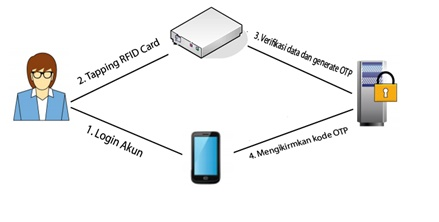
\includegraphics[width=8cm]{figures/Masuk.jpg}
\end{center}
\caption{(IN) Process.
\label{eq:30}}
\end{figure}  

\subsubsection{OUT Process} 
In the process (OUT) consists of 4 steps, namely:

\begin{enumerate}
    \item 
    User Login Account to local system via a smartphone device.
    \item
     User tapping RFID card
    \item 
    User Entering the existing OTP code and the system will verify the RFID ID and the inputted OTP code.
    \item
    If appropriate, Data Successfully saved.
\end{enumerate}
\begin{figure}[ht]
\begin{center}
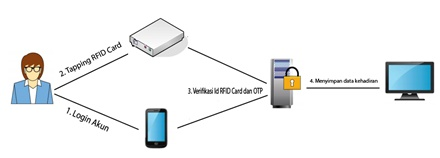
\includegraphics[width=8cm]{figures/Keluar.jpg}
\end{center}
\caption{(OUT) Process.
\label{eq:30}}
\end{figure} 

\section{Experiment}
\label{Experiment}
The experiment is performed to determine the function and performance of the whole system. The experiment program is simulated in a suitable system. This experiment is conducted to determine the reliability of the system and to determine whether it is in accordance with the planning or not. The experiment will be done that is in accordance with the step steps in Figure 1 and Figure 2.

\subsection{Hardware Used}
The modules have been compiled with all the required sequences and have been implemented with the required components. The overall design result of the tool and system can be seen in the following figure:
\begin{figure}[ht]
\begin{center}
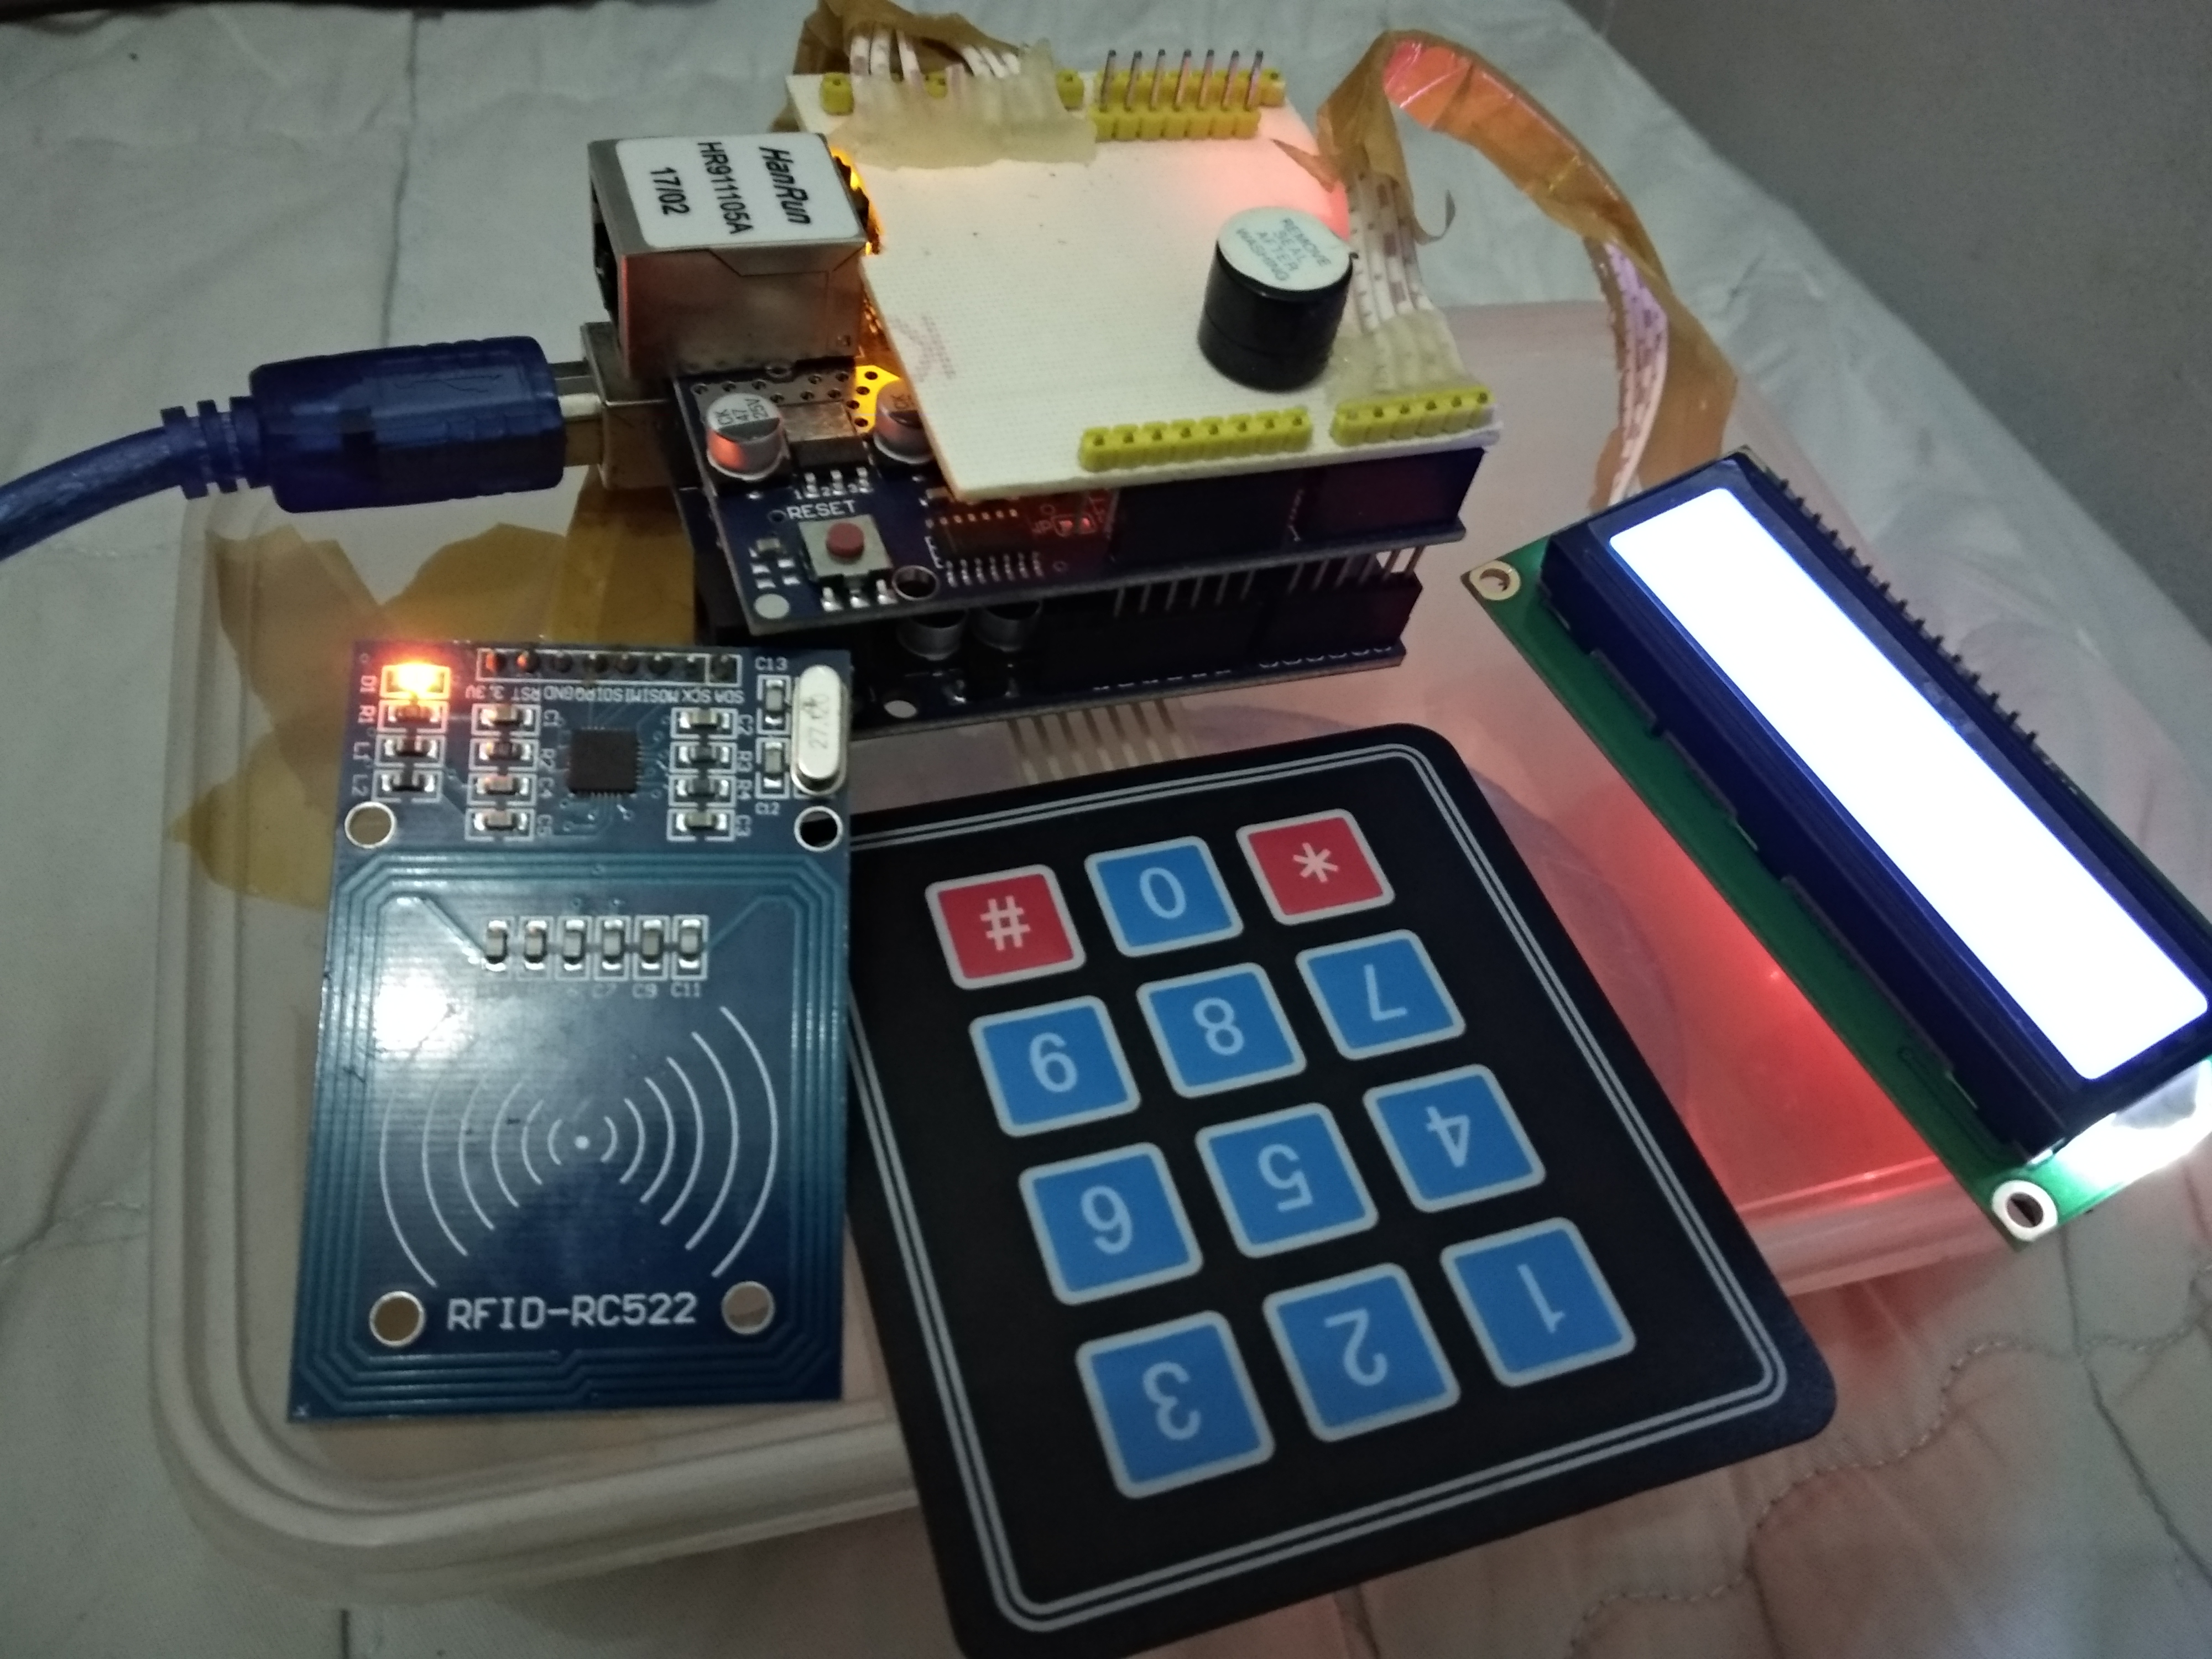
\includegraphics[width=8cm]{figures/Tools.jpg}
\end{center}
\caption{RFID Tools.
\label{eq:30}}
\end{figure} 

\subsection{Implementation Methods}
The application of the Multi-Factor Authentication method with the implementation of the OTP code is used to secure and verify the user. With this method user authentication will be performed.
The process of applying the method on this hardware is when the user tapping in the morning or early entry to work then the code will be sent to the user account based on the card ID, then when the clock home has arrived the user will do tapping and input the code on the keypad that has been provided.
After entering the OTP code 'hash' button on the keypad is pressed to transmit data and check the code in the database.

\begin{left}
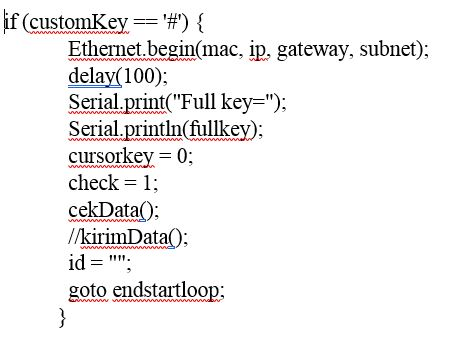
\includegraphics[width=6cm]{figures/COde1.JPG}
\end{left}

If wrong inserts the OTP key 'star' key on the keypad is pressed to delete the wrong number

\begin{left}
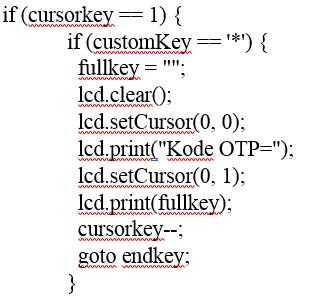
\includegraphics[width=4.5cm]{figures/COde2.JPG}
\end{left}


\subsection{Working of The System}
The concatenation in Figure 3 will be tested to perform user authentication process that is by way of initial entry, user will tapping rfid card to rfid reader. If the card has been registered with the OTP code will be sent to the user's account and the clock data entry will be stored on the database. And If the curfew, the user will be tapping an RFID card again and enter the code OTP had previously been sent to the account. Users will enter OTP code with a keypad that has been provided, if the code OTP appropriate then clock out successfully saved to the database, if it fails you will be notified if the code is entered incorrectly OTP.

If the card is not registered then the OTP code can not be sent and on the LCD will show the notification that the card used is not listed.

\begin{left}
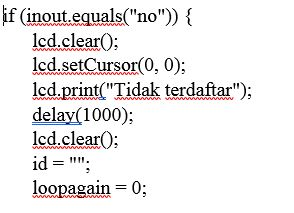
\includegraphics[width=5cm]{figures/COde3.JPG}
\end{left}

Furthermore, if the card is already registered but not feeding the notification that the OTP code is incorrect.

\begin{left}
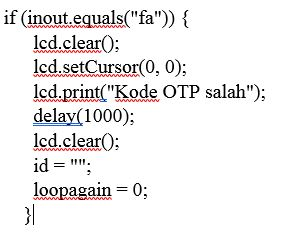
\includegraphics[width=4.5cm]{figures/COde4.JPG}
\end{left}

Therefore the system and Hardware will be interconnected with each other. Namely connected using ethernet and access to the system using the IP address is: 192.168.1.102.

\begin{left}
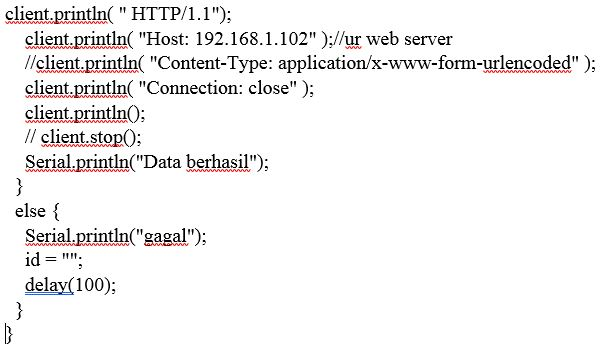
\includegraphics[width=8cm]{figures/COde5.JPG}
\end{left}

\section{Result}
\label{Result}
Based on the experimental results that have been applied the application of the method has been successfully applied.
From the experimental results obtained:
\begin{enumerate}
    \item 
    if the card has not been registered then the card can not be read by system and will notification "Card is not Register".
    \item
    If the inserted OTP code does not match the code sent to the feeding user's account it will be rejected by the system and on the LCD it will display the notification of 'Invalid OTP Code'.
    \item
    If the OTP code and the card is in accordance then the data will be stored and the LCD will show the notification 'Thank you'
    \item
    The system can only be accessed using a predefined IP that is 192.168.1.102
    \item
    OTP code will be different every day and will be automatically generated when user tapping.
\end{enumerate}

Here are the results of the OTP code that was successfully sent to the user's account or card owner.
\begin{figure}[ht]
\begin{center}
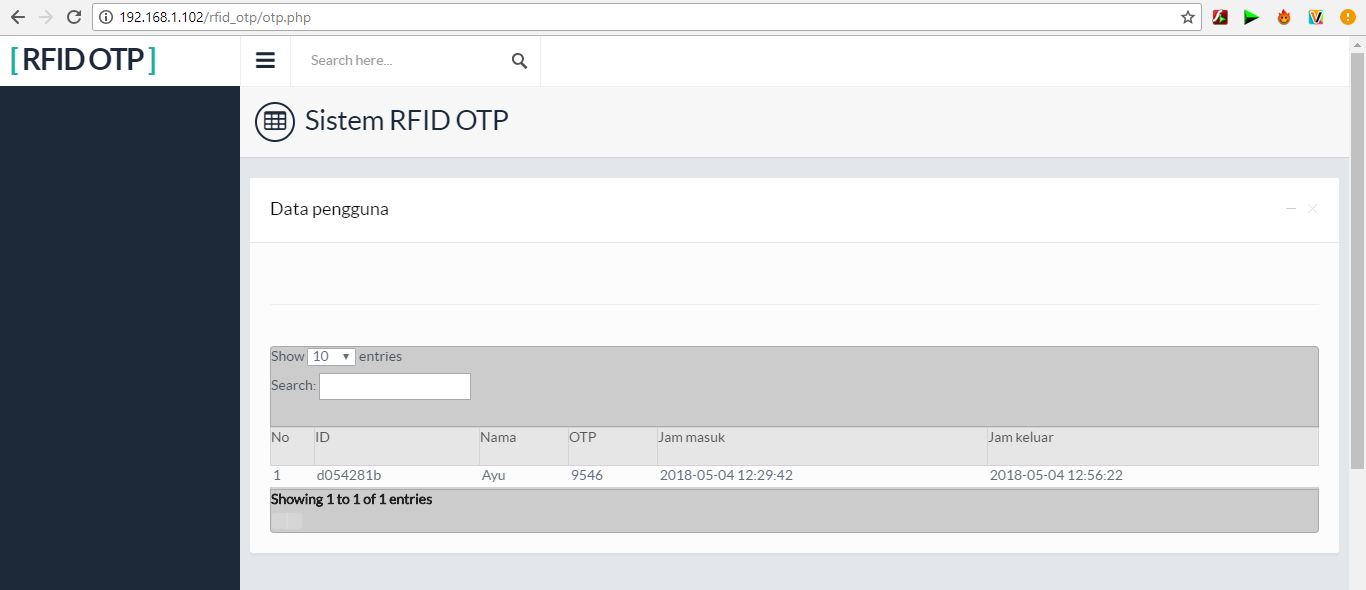
\includegraphics[width=12cm]{figures/OTP1.JPG}
\end{center}
\caption{User Account.
\label{eq:30}}
\end{figure}  

\begin{figure}[ht]
\begin{center}
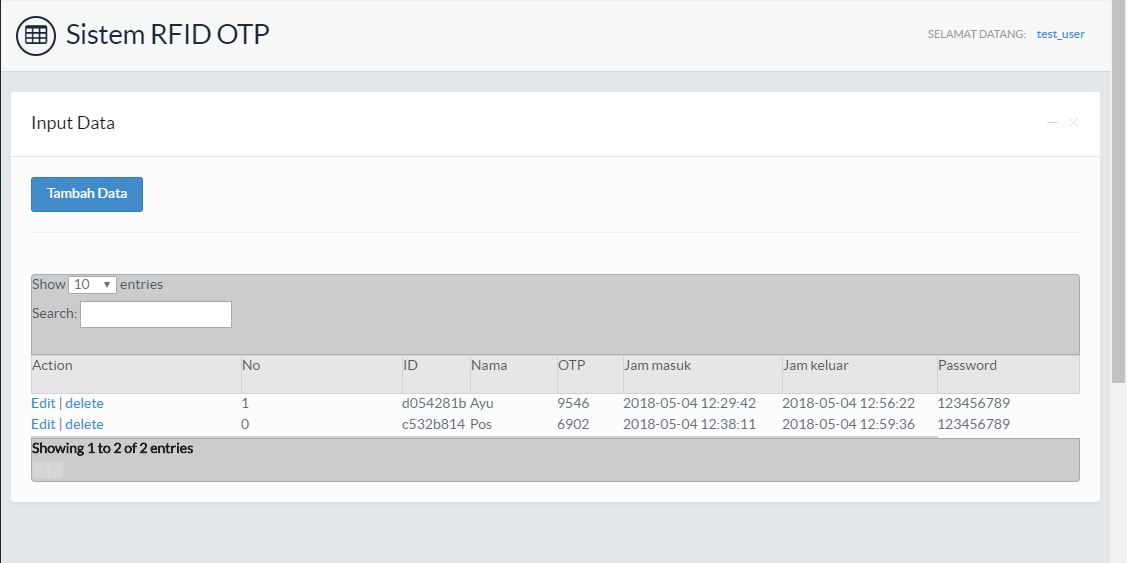
\includegraphics[width=12cm]{figures/AdminOTP.JPG}
\end{center}
\caption{Admin.
\label{eq:30}}
\end{figure}  




\section{Conclusion}
\label{Conclusion}
Based on the results of experiments that have been done show that, by utilizing the method of Multi-Factor Authentication to make the existing system becomes more secure by performing several steps of authentication. Each user has a card each and on the card has different IDs. Every day while tapping, users will get an OTP Authentication code. The code will be sent to each user account. The OTP code will be used at home from work. Users will tapping and entering the code that has been sent. If the code is appropriate then the data will be updated and stored into the data base. But if it is wrong then the data will not be stored, and will be rejected by the system. Likewise when the card used is not registered in the database. System can be accessed through IP that has been provided. So with the system by using some steps of this authentication can minimize the occurrence of duplication of RFID card and minimize the occurrence of cheating that will happen later.

\section{Discussion}
\label{Discussion}
Based on the results of experiments that have been done show that, by utilizing the method of Multi-Factor Authentication to make the existing system becomes more secure by performing several steps of authentication. Each user has a card each and on the card has different IDs. Every day while tapping, users will get an OTP Authentication code. The code will be sent to each user account. The OTP code will be used at home from work. Users will tapping and entering the code that has been sent. If the code is appropriate then the data will be updated and stored into the data base. But if it is wrong then the data will not be stored, and will be rejected by the system. Likewise when the card used is not registered in the database. System can be accessed through IP that has been provided. So with the system by using some steps of this authentication can minimize the occurrence of duplication of RFID card and minimize the occurrence of cheating that will happen later.

\bibliographystyle{IEEEtran}
\bibliography{references}


\end{document}
